
\documentclass{ifacconf}

% Pre-load natbib in the preamble. ifacconf.cls otherwise \RequirePackage{natbib}s
% inside \AtBeginDocument, which fires natbib's own \AtBeginDocument{\NAT@set@cites}
% before \NAT@idxtxt is defined and crashes a clean build (no stale .aux). Loading it
% here lets natbib.sty finish before any begin-document hook runs; ifacconf's later
% \RequirePackage is then a no-op and still sets \bibliographystyle{ifacconf}.
\usepackage{natbib}

\usepackage{url}
\usepackage{graphicx} % for pdf, bitmapped graphics files
\usepackage{graphicx}
\usepackage{amsmath} % assumes amsmath package installed
\usepackage{amssymb}  % assumes amsmath package installe
\usepackage{booktabs}
\usepackage{mathrsfs}
\usepackage{tikz}
\usepackage{pifont}
\usetikzlibrary{arrows.meta}
% --- Removed for portable local compilation (uninstalled/unneeded on the build box):
% algorithm, algpseudocode, wrapfig, latexsym, pst-text/node/plot, dsfont, auto-pst-pdf.
% amsthm is NOT loaded: ifacconf.cls already provides \newtheorem + the proof env and
% loads natbib. ---
\usepackage{amsmath,amssymb}
\usepackage{caption}
\usepackage{float}
\usepackage{bm}
\usepackage{multirow}
\usepackage{subfig}
\usepackage{verbatim}
%\usepackage{tabls}
% NOTE: do NOT load \usepackage{cite} — ifacconf.cls auto-loads natbib (author-year,
% ifacconf.bst). Use \citet{}/\citep{} for citations. (cite conflicts with natbib.)
% \usepackage{hyperref}
\usepackage{comment}
\usepackage{amsmath}

\usetikzlibrary{shapes,arrows,chains,matrix,positioning,scopes,shadows,calc}
%\usetikzlibrary{decorations.pathmorphing,decorations.pathreplacing,decorations.shapes}
\newtheorem{theorem}{Theorem}

\newtheorem{lemma}{Lemma}
\newtheorem{proposition}{Proposition}
\newtheorem{corollary}{Corollary}
\newtheorem{definition}{Definition}
\newtheorem{assumption}{Assumption}
\newtheorem{remark}{Remark}
% Bold theorem-like headers (Lemma 1, Proposition 1, ...) instead of the class default
% italic, for clearer visual anchors (standard in control/math papers). The statement text
% and the parenthetical title keep the class defaults.
\makeatletter
\def\theorem@headerfont{\normalfont\bfseries}
\makeatother
% proof environment (ifacconf does not provide one; amsthm was removed to avoid a clash)
\newenvironment{proof}{\par\noindent{\itshape Proof.}\space}{%
  \unskip\nobreak\hfil\penalty50\hskip1em\null\nobreak\hfil$\square$%
  \parfillskip=0pt\finalhyphendemerits=0\par\addvspace{2pt}}
\newcommand\scalemath[2]{\scalebox{#1}{\mbox{\ensuremath{\displaystyle #2}}}}
% placeholder box for figures added later (keeps the document compiling with no media files)
\newcommand{\figph}[2]{\fbox{\begin{minipage}[c][#2][c]{#1}\centering\footnotesize\ttfamily[\,figure to be added\,]\end{minipage}}}
% mark-less footnote (for the equal-contribution note; the dagger in the text matches the author markers)
\newcommand\blfootnote[1]{\begingroup\renewcommand\thefootnote{}\footnotetext{#1}\endgroup}
\usepackage[font=small,labelfont=bf]{caption}

% \usepackage{calrsfs}  % removed (\pazocal unused)
% \DeclareMathAlphabet{\pazocal}{OMS}{zplm}{m}{n}

\usepackage{color}
%\usepackage{subcaption}
% \renewcommand{\blacksquare}{\qed}  % removed: \qed not defined without amsthm
\newcommand{\cb}{\color{blue}}
\newcommand{\cd}{\color{red}}
\newcommand{\cred}{\color{red}}



\newcommand{\Ln}{L_\Delta}
\newcommand{\kron}{\otimes}

\DeclareMathOperator{\tr}{tr}
% \newcommand{\Rset}{\mathbb{R}}

\newcommand{\RESsolvesCone}{\ensuremath{797\pm16}}\newcommand{\RESsolvesCthree}{\ensuremath{32\pm1}}
\newcommand{\RESmsCone}{\ensuremath{3.9\pm0.1}}\newcommand{\RESmsCthree}{\ensuremath{7.9\pm0.4}}
\newcommand{\REScpuCone}{\ensuremath{3123\pm56}}\newcommand{\REScpuCthree}{\ensuremath{253\pm6}}
\newcommand{\RESoffCone}{\ensuremath{0.128\pm0.002}}\newcommand{\RESoffCthree}{\ensuremath{0.060\pm0.005}}
\newcommand{\REScov}{\ensuremath{0.0095}}\newcommand{\RESsolveRed}{25}\newcommand{\REScpuRed}{12}
% reproducibility: identical-config UGV ground-truth path fork
\newcommand{\RESforkGUI}{2.7}\newcommand{\RESforkHL}{0.03}
% Altitude-policy comparison (hairpin, headless, GSD noise, R=3): adaptive vs fixed-low(2.5) vs fixed-high(7).
% mean/max estimation covariance tr(Sigma); each fixed policy is dominated on one axis.
\newcommand{\RESaltAdaptMean}{\ensuremath{0.0065}}\newcommand{\RESaltLowMean}{\ensuremath{0.0062}}\newcommand{\RESaltHiMean}{\ensuremath{0.0105}}
\newcommand{\RESaltAdaptMax}{\ensuremath{0.016}}\newcommand{\RESaltLowMax}{\ensuremath{0.14}}\newcommand{\RESaltHiMax}{\ensuremath{0.030}}
\newcommand{\RESaltHiPen}{61}\newcommand{\RESaltLowRatio}{9}
\newcommand{\RESaltLo}{2.5}\newcommand{\RESaltHiZ}{5.1}
% The long title needs the full text width to set on two lines, but the author block,
% address, and abstract must stay in the default (narrower) centered front-matter column.
% So we widen ONLY the title: typeset it in a full-\textwidth box centered on the
% (page-centered) front-matter column, leaving everything else untouched. This lives
% entirely in the document preamble and does NOT modify ifacconf.cls.
\makeatletter
\def\title@fmt#1#2{%
  \@ifundefined{@runtitle}{\global\def\@runtitle{#1}}{}%
  \@articletypesize
  \leavevmode\vphantom{Aye!}%
  \@articletype
  \vskip12\p@
  % \kern\@frontindent shifts the full-width title parbox right so it is page-centered,
  % matching the author/address lines (which the class centers via a \@frontindent leftskip).
  {\hfuzz\maxdimen\hbox to\hsize{\kern\@frontindent\hss
     \parbox{\textwidth}{\centering\@titlesize #1\,\hbox{$^{#2}$}\par}\hss}}%
  \vskip\@undertitleskip
}
\makeatother
%===============================================================================
\begin{document}
\begin{frontmatter}

\title{COAST: Altitude as a Coupled Perception Variable\\ in Shared-Camera Aerial-Ground Tracking}
% Title, preferably not more than 10 words.

\author[First]{Shlok Mehndiratta$^{\dagger}$}
\author[First]{Prashant Gupta$^{\dagger}$} 
\author[First]{Divyam Sood$^{\dagger}$} 
\author[First]{Agniva Banerjee} 
\author[First]{Arijit Sen}
\address[First]{Department of Electrical Engineering and Computer Science, IISER Bhopal, India. (e-mail: \{shlokm23, prashant23, divyam23, agniva24, ajsen\}@iiserb.ac.in).}

\begin{abstract}
This paper considers a shared-camera aerial-ground tracking problem by a UAV and a UGV system. We assume
that a single downward-facing UAV camera is the sole exteroceptive sensor of the UGV, which serves as its
navigation reference through lane segmentation. This shared sensor couples navigation and estimation
through the UAV altitude $z$, which sets localization resolution (the measurement-noise covariance $R$
grows as $R\propto z^2$) and navigation coverage (the camera footprint) in opposite directions, since
raising the altitude improves coverage but coarsens resolution while lowering it does the reverse. We treat
altitude as a variable to be optimized and solve the coupling in closed form: the best altitude for
estimation is the lowest one that still keeps the path inside the camera footprint, and because a sharper
turn needs a longer look-ahead, this lowest admissible altitude increases with path curvature. Adapting
altitude along the path improves estimation over any single fixed altitude only when this admissible
altitude is active and the curvature changes; otherwise a fixed altitude performs equally well. We deploy
the proposed policy, COAST (Coupled-Altitude Shared-camera Tracking), which commands the UAV to fly at this
curvature-scheduled altitude, together with a belief-space ground controller and a perception-triggered
aerial planner whose ancillary law is shown to keep the inter-trigger tracking error bounded and free of
Zeno behavior. A reproducible ROS\,2/Gazebo study confirms each prediction: the measured sensor noise
follows $R\propto z^2$; the steady-state estimation cost increases monotonically with altitude and does not
depend on the track; the adaptive policy matches the best fixed altitude on our testbed; and
event-triggering the aerial planner reduces its computation by more than an order of magnitude at the same
estimation quality.
\end{abstract}

\begin{keyword}
Perception-aware control, Cooperative aerial-ground systems, Belief-space planning,
Event-triggered control, Estimation and Kalman filtering
\end{keyword}

\end{frontmatter}

\section{Introduction}
\label{sec:intro}
\blfootnote{$^{\dagger}$~denotes equal contribution.}

Unmanned ground vehicles (UGVs) operating in unstructured or GPS-denied environments are limited by short
and occlusion-prone perception horizons, as onboard LiDAR and stereo cameras have a narrow field of view
and cannot see far enough ahead to anticipate the upcoming path \citep{frey2024roadrunner}.
A now-standard remedy is aerial-ground cooperation, in which an unmanned aerial vehicle (UAV) acts as an
elevated eye for the perception-limited ground robot \citep{grocholsky2006cooperative,li2024colag,santos2024aerial}.
However, most of such systems hold the UAV at a fixed altitude and never treat that altitude as a decision
variable. The aerial vehicle follows a distance-minimizing trajectory and returns the state estimates of
ground robot as a downstream byproduct. This decoupling is fragile. When the ground robot maneuvers sharply
or is briefly occluded, the estimation covariance grows and tracking degrades, which is not desired.

We begin instead from a structural observation about the shared sensor. When a single downward-facing
camera on the UAV is the ground robot's only exteroceptive sensor, one image serves two roles at once: the
lane ahead is segmented into a navigation waypoint, and a marker on the robot is detected into a noisy pose
measurement for the estimator. Because both products are read from the same image, they share the same
imaging geometry, and in particular the same altitude. Raising the camera enlarges the ground footprint and
improves navigation coverage, but it coarsens the ground sampling distance and inflates the localization
noise, whose covariance $R$ grows with the camera altitude $z$ as $R\propto z^2$; lowering it does the
reverse. Therefore, a single scalar, the UAV altitude, sets estimation resolution and navigation coverage
simultaneously but in competition, so that the altitude best for one is worst for the other. This
antagonism turns altitude from a geometric parameter into an active perception variable, and characterizing
how to use it is the subject of this paper.

This viewpoint connects to two established lines of work, and departs from both in the same place.
Perception-aware trajectory optimization shapes a robot's own motion to serve estimation, through the
sensor trajectory \citep{falanga2018pampc,spasojevic2020perception} and viewpoint selection
\citep{zhang2019fisher}, while belief-space planning and active SLAM go further, augmenting the planning
state with the estimator covariance to act deliberately under partial observability
\citep{platt2010belief,vandenberg2012motion,placed2023survey}.
Our ground-robot controller belongs to this belief-space family. The novelty is that it allows to guarantee
where the information decision lives and what it trades. In these aforementioned works a robot reshapes its
own trajectory to see better. On contrary in our controller, the decisive variable is a teammate's
altitude, and it sets two perception products against each other rather than sharpening one. That altitude
alone trades localization resolution against sensor coverage is itself known, and has been exploited to
balance a coverage-quality criterion in multi-UAV area coverage \citep{papatheodorou2017coverage} and to
meet resolution constraints in photogrammetric coverage planning \citep{difranco2016coverage}. To our
knowledge, the closed-loop \emph{shared-camera} instantiation has not yet been formulated, where one
downward camera is the ground robot's only exteroceptive sensor and the same altitude is used as an EKF
measurement (favoring low $z$) and in lane-segmentation coverage (favoring higher $z$). For this coupling,
we give a closed-form solution of curvature-scheduled optimal altitude, which is characterized with
adaptation. Quadrotor target-tracking under limited field-of-view and occlusion is likewise well studied
\citep{thomas2017autonomous,penin2018vision}. However, the coverage-versus-accuracy trade is split across
separate robots or sensors and the altitude is held fixed rather than optimized.

Deploying the resulting policy in closed loop additionally demands robust tracking
under bounded disturbances and a bounded compute budget. Tube MPC supplies the first, decomposing control
into a nominal plan and an ancillary law that confines the error to a robust positively invariant tube
\citep{mayne2005robust,mRPI}, and event-triggered
control supplies the second, re-solving only when a state-dependent condition fires
\citep{tabuada2007event,li2014event}. Both are conventionally driven
by a fixed disturbance set and a purely state-based condition. We drive the trigger by perception instead,
using the estimator covariance, whose closest precedent is variance-based triggering for state estimation
\citep{trimpe2014event}, together with the anticipated path curvature, and we certify the resulting
inter-trigger behavior.

Building on these observations, we develop COAST, which treats altitude as a coupled perception variable,
and make three contributions:
\begin{itemize}
\item \emph{The coupling and its regime (Section~\ref{sec:method}).} We formalize the shared-camera
altitude coupling and solve it in closed form. The best altitude for estimation is the lowest one that
keeps the path within the camera footprint, and it rises with path curvature; adapting altitude along the
path beats every fixed altitude exactly when this lowest admissible altitude is active and the curvature
varies, and otherwise a single fixed altitude is already optimal. The contribution is this characterization
of \emph{when} adaptation helps, not a claim that it always helps.
\item \emph{An event-triggered co-design.} We deploy the policy with a belief-space ground controller and a
perception-triggered aerial planner whose ancillary law is shown to be input-to-state stable between two
consecutive triggers and free of Zeno behavior, which makes perception-aware replanning affordable on a
constrained companion computer.
\item \emph{A reproducible SITL study.} We build a complete ROS\,2/Gazebo testbed under one per-step
logging protocol and use it to verify each analytical prediction; the code and data are publicly
available.\footnote{\url{https://github.com/soododivyam/COAST-public-release}}
\end{itemize}
Figure~\ref{fig:testbed} shows the testbed and the single camera in its dual role.

\begin{figure}[htbp]
\centering
\subfloat[Downward View]{\label{fig:cmera}
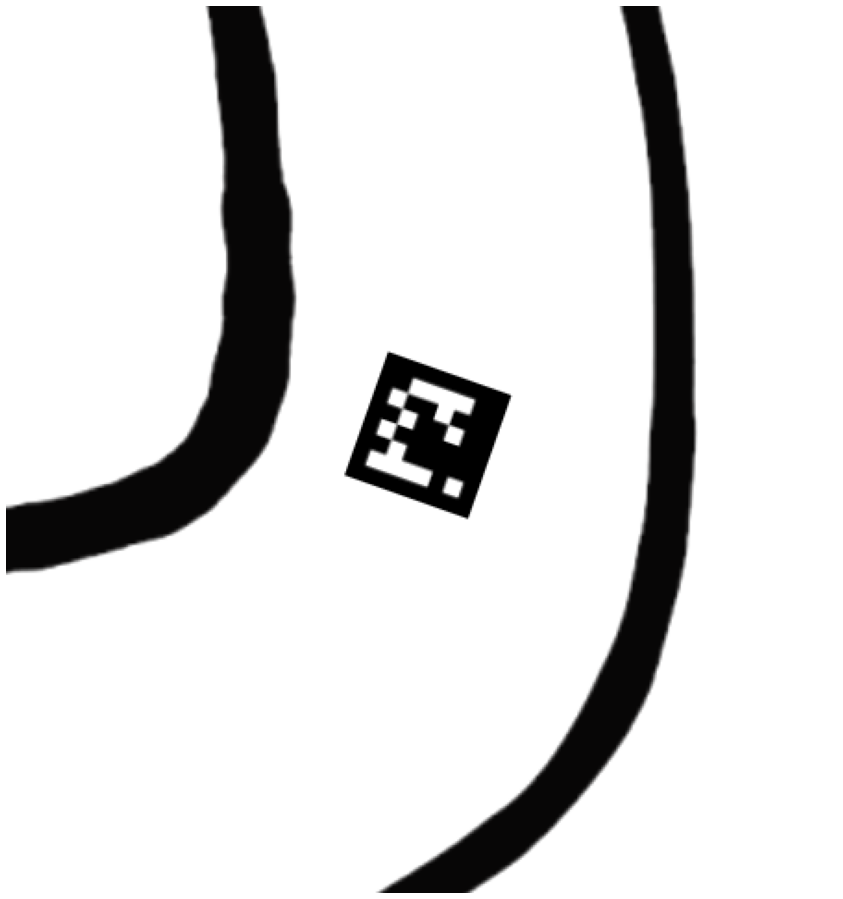
\includegraphics[width=3.5cm]{media/Fig_Testbed1.png}
}\hfil
\subfloat[Dual Role]{\label{fig:frame}
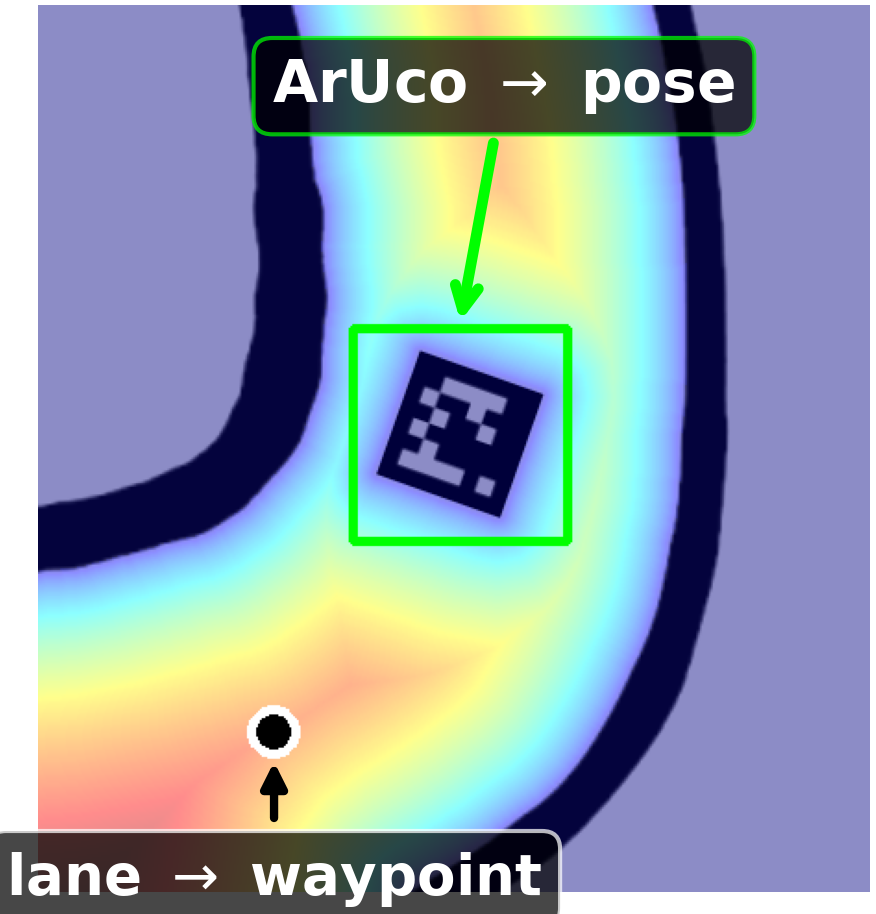
\includegraphics[width=3.5cm]{media/Fig_Testbed2.png}
}
\caption{The single downward-facing camera in its dual role. (a) the aerial view of the marked UGV on its
lane. (b) the same frame yields both a navigation waypoint (from the segmented lane) and the EKF pose
measurement (from the ArUco marker).}
\label{fig:testbed}
\end{figure}


\section{System Modeling and Problem Formulation}
\label{sec:model}
A UAV tracks a UGV in a common world frame $\mathcal{F}_W$. The UAV carries the system's
\emph{only} exteroceptive sensor, a single downward-facing monocular camera, while the UGV is
otherwise perception-limited, equipped only with wheel odometry. Each camera frame yields two
products (Fig.~\ref{fig:system}): the lane ahead of the vehicle, segmented to produce a navigation
waypoint, and an ArUco fiducial marker \citep{garridojurado2014aruco} on the UGV, detected to produce a
noisy pose measurement. The pose measurement is fused with odometry in an extended Kalman filter (EKF),
yielding a belief $(\mu,\Sigma)$, that is, a mean $\mu$ and covariance $\Sigma$ over the UGV state.

Because both products are read from the same image, they share the same altitude, which therefore sets
estimation quality and navigation coverage together but in competition: a higher altitude improves
coverage while coarsening resolution, and a lower altitude does the reverse. The remainder of this
section formalizes the two sides of this coupling through the vehicle motion, resolution, and coverage
models, and states the constrained estimation problem they induce, which Section~\ref{sec:method} solves.

\begin{figure}[t]
\centering
\resizebox{\columnwidth}{!}{%
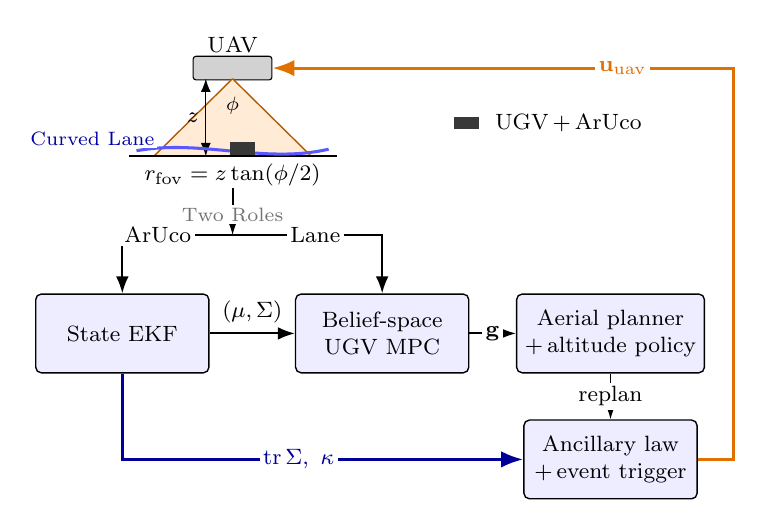
\begin{tikzpicture}[font=\small,>=Latex,
  blk/.style={draw,rounded corners=2pt,align=center,minimum height=10mm,minimum width=22mm,
              inner sep=3pt,fill=blue!7,line width=0.5pt,font=\footnotesize},
  sig/.style={->,line width=0.7pt},
  cpl/.style={->,line width=1.1pt,blue!60!black},
  fb/.style={->,line width=1.1pt,orange!88!black},
  lab/.style={font=\footnotesize,fill=white,inner sep=1.3pt},
  slab/.style={font=\scriptsize,fill=white,inner sep=1pt}]

% ===================== physical scene (top) =====================
\begin{scope}[shift={(1.85,0)}]
  \node[draw,fill=gray!35,minimum width=10mm,minimum height=3mm,rounded corners=1pt] (uav) at (0,1.62) {};
  \node[font=\footnotesize] at (0,1.92) {UAV};
  \coordinate (cam) at (0,1.485);
  % field-of-view cone
  \fill[orange!16] (cam) -- (-1.0,0.5) -- (1.0,0.5) -- cycle;
  \draw[orange!70!black,line width=0.5pt] (cam)--(-1.0,0.5);
  \draw[orange!70!black,line width=0.5pt] (cam)--(1.0,0.5);
  \node[font=\scriptsize] at (0,1.14) {$\phi$};
  % altitude (left of the optical axis)
  \draw[<->] (-0.34,0.5)--(-0.34,1.485) node[midway,left=-1pt,font=\footnotesize]{$z$};
  % ground + curved lane
  \draw[line width=0.8pt] (-1.32,0.5)--(1.32,0.5);
  \draw[blue!65,line width=1.1pt] (-1.22,0.57) .. controls (-0.4,0.72) and (0.4,0.4) .. (1.22,0.59);
  \node[slab,text=blue!65!black,anchor=east] at (-0.95,0.72) {Curved Lane};
  % UGV on the ground (labelled in the top-right legend, to keep the FoV area clean)
  \fill[black!78] (-0.03,0.52) rectangle (0.29,0.68);
  % footprint radius
  \draw[|<->|] (-1.0,0.26)--(1.0,0.26)
     node[midway,fill=white,inner sep=1pt,font=\footnotesize]{$r_{\mathrm{fov}}=z\tan(\phi/2)$};
\end{scope}

% ===================== block diagram (bottom) =====================
\node[blk] (ekf)    at (0.45, -1.75) {State EKF};
\node[blk] (ugvmpc) at (3.75, -1.75) {Belief-space\\UGV MPC};
\node[blk] (plan)   at (6.65, -1.75) {Aerial planner\\+\,altitude policy};
\node[blk] (anc)    at (6.65, -3.35) {Ancillary law\\+\,event trigger};
% legend: the black rectangle in the scene is the marked UGV (same shape as in the scene)
\fill[black!78] (4.66,0.84) rectangle (4.98,1.00);
\node[font=\footnotesize,anchor=west] at (5.06,0.92) {UGV\,+\,ArUco};

% one camera image -> two roles (fan out from below the camera)
\draw[sig] (1.85,0.10) -- (1.85,-0.5) coordinate (fork);
\draw[sig] (fork) -| (ekf.north);
\draw[sig] (fork) -| (ugvmpc.north);
\node[lab] at (0.9,-0.5) {ArUco};
\node[lab] at (2.9,-0.5) {Lane};
\node[slab,text=black!55] at (1.85,-0.24) {Two Roles};

% belief into the UGV controller; plan and re-plan
\draw[sig] (ekf.east) -- (ugvmpc.west) node[midway,above=0pt,font=\footnotesize]{$(\mu,\Sigma)$};
\draw[sig] (ugvmpc.east) -- (plan.west) node[lab,midway]{$\mathbf{g}$};
\draw[sig] (plan.south) -- (anc.north) node[lab,midway]{replan};

% coupling: covariance and curvature drive the trigger
\draw[cpl] (ekf.south) |- (anc.west) node[lab,pos=0.72]{$\mathrm{tr}\,\Sigma,\ \kappa$};

% feedback: the UAV command closes the loop through the physical UAV
\draw[fb] (anc.east) -- ++(0.45,0) |- (uav.east) node[lab,pos=0.62]{$\mathbf{u}_{\mathrm{uav}}$};

\end{tikzpicture}}

\caption{System overview. The UAV at altitude $z$ views the ArUco-tagged UGV within the footprint
$r_{\mathrm{fov}}=z\tan(\phi/2)$, so altitude sets both localization resolution and coverage. The single
image yields two products: a lane waypoint and an ArUco pose for the EKF, whose belief $(\mu,\Sigma)$ and
the waypoint drive the belief-space UGV MPC; its predicted endpoint $\mathbf{g}$ drives the aerial planner
and altitude policy, and the ancillary law and event trigger return the command $\mathbf{u}_{\mathrm{uav}}$
that closes the loop. Blue: the covariance $\mathrm{tr}\,\Sigma$ and curvature $\kappa$ drive the trigger.}
\label{fig:system}
\end{figure}

\subsection{Vehicle models}
\label{sec:vehicles}
The UGV follows unicycle kinematics with first-order actuator lag. Its state is
$\mathbf{x}_g=[x_g,y_g,\theta,v,\omega]^{\!\top}$, collecting the planar position $(x_g,y_g)$, the
heading $\theta$, and the linear and angular rates $(v,\omega)$; the commanded velocities are
$\mathbf{u}_g=[v_c,\omega_c]^{\!\top}$. The discrete-time model is
\begin{equation}
\mathbf{x}_{g,k+1}=\mathbf{f}_g(\mathbf{x}_{g,k},\mathbf{u}_{g,k})+\mathbf{w}_g,
\label{eq:ugv}
\end{equation}
where the map $\mathbf{f}_g$ integrates the unicycle kinematics, the actuators track their commands
through first-order lags of time constants $\tau_v,\tau_\omega$, and $\mathbf{w}_g$ is a bounded
process noise. The heading and rate states are retained because the marker yields a full planar pose,
not merely a position, which the estimator exploits.

The UAV is a quadrotor, but the planning and tracking layers treat it as a velocity-controlled point
mass; an inner-loop attitude and thrust controller (in our study, the Gazebo velocity-control plugin)
is assumed to realize the commanded velocities. Writing the UAV position as
$\mathbf{p}=[p_x,p_y,p_z]^{\!\top}$, the altitude as $z:=p_z$, and the velocity command as
$\mathbf{u}=[v_x,v_y,v_z]^{\!\top}$, the single-integrator model is
\begin{equation}
\mathbf{p}_{k+1}=\mathbf{p}_k+\Delta t\,\mathbf{u}_k+\mathbf{w}_k,\qquad A_d=I_3,\quad B_d=\Delta t\,I_3,
\label{eq:uav_disc}
\end{equation}
with sampling period $\Delta t$, state matrix $A_d=I_3$ (the $3\times3$ identity), input matrix
$B_d=\Delta t\,I_3$, and bounded disturbance $\mathbf{w}_k\in\mathbb{W}$. All three axes are actuated,
so the vertical velocity $v_z$ is a genuine decision variable and the altitude is commanded in closed
loop. The linear form of \eqref{eq:uav_disc} makes the ancillary error dynamics exact, which
Section~\ref{sec:method} uses in the event-triggered controller.

\subsection{Resolution model}
\label{sec:resolution}
The accuracy of marker-based localization is set by the camera's ground sampling distance (GSD), the
metric size of one pixel on the ground, which grows linearly with altitude. If the image-plane
detection error is approximately constant in pixels, the metric position error grows in proportion to
the GSD, so the position-measurement covariance grows quadratically with altitude. Let $z_0$ be a
reference altitude, $d=\lVert\mathbf{p}^{xy}-\mathbf{p}_g\rVert$ the horizontal UAV--UGV separation
(with $\mathbf{p}^{xy}$ the UAV's planar position and $\mathbf{p}_g$ the UGV's), $\phi$ the camera
field of view, and $r_{\mathrm{fov}}(z)=z\tan(\phi/2)$ the resulting footprint radius. We model the
measurement covariance as
\begin{equation}
R(z)=R_0\!\left(\frac{z}{z_0}\right)^{\!2}\!\left(1+\Big(\frac{d}{r_{\mathrm{fov}}}\Big)^{\!2}\right),
\label{eq:Rgsd}
\end{equation}
where $R_0$ is the baseline covariance at $z_0$, the factor $(z/z_0)^2$ is the GSD scaling, and the
factor $1+(d/r_{\mathrm{fov}})^2$ mildly inflates the noise as the target approaches the footprint
edge (loss of accuracy away from the optical axis). Equation~\eqref{eq:Rgsd} is strictly increasing
in $z$; this monotonicity is the resolution side of the coupling. The scaling is not merely
postulated; it is measured directly in Section~\ref{sec:results}. The same model \eqref{eq:Rgsd}
drives both the EKF and the belief-space planner of Section~\ref{sec:method}.

\subsection{Coverage model}
\label{sec:coverage}
Lane segmentation seeds a waypoint a lookahead distance ahead of the vehicle, and that waypoint must
fall inside the footprint or the reference is lost. Writing the required lookahead as
$d_{\mathrm{look}}(\kappa)$, which grows with the local path curvature $\kappa$ (a curving lane
leaves the footprint sooner), we summarize navigability by the non-dimensional \emph{coverage factor}
\begin{equation}
\eta(z,\kappa)=\frac{r_{\mathrm{fov}}(z)}{d_{\mathrm{look}}(\kappa)}=\frac{z\tan(\phi/2)}{d_{\mathrm{look}}(\kappa)},
\label{eq:eta}
\end{equation}
with segmentation feasible for $\eta\ge 1$, equivalently $z\ge z_{\mathrm{fl}}(\kappa):=
d_{\mathrm{look}}(\kappa)/\tan(\phi/2)$. This altitude \emph{floor} $z_{\mathrm{fl}}(\kappa)$ is the
coverage side of the coupling, and it opposes the resolution side directly: the estimator prefers
\emph{low} altitude for resolution \eqref{eq:Rgsd}, whereas \eqref{eq:eta} demands \emph{sufficient}
altitude for coverage, and the floor rises exactly where the path curves.

\subsection{Problem formulation}
\label{sec:problem}
Together the resolution and coverage models pose an altitude-selection problem. Over a traversal of
duration $T$ with curvature profile $\kappa(t)$, define the time-averaged estimation cost
\begin{equation}
J[z(\cdot)]=\frac{1}{T}\int_0^T \operatorname{tr}P_\infty\!\big(R(z(t))\big)\,dt,
\label{eq:Jest}
\end{equation}
where $P_\infty(R)$ is the steady-state estimation-error covariance under measurement noise $R$
(made precise in Section~\ref{sec:method}) and $\operatorname{tr}(\cdot)$ is the trace. The
\emph{altitude-selection problem} is
\begin{equation}
\min_{z(\cdot)}\ J[z(\cdot)]\quad\text{s.t.}\quad z(t)\ge z_{\mathrm{fl}}(\kappa(t)),\ \ z(t)\in[z_{\min},z_{\max}],
\label{eq:altprob}
\end{equation}
that is, minimize the estimation cost subject to coverage feasibility and the actuation limits
$[z_{\min},z_{\max}]$. Alongside \eqref{eq:altprob}, the deployed system must (i) keep the UGV within
the footprint so that $\Sigma$ stays bounded, (ii) track the UGV robustly under the bounded
disturbance set $\mathbb{W}$, and (iii) limit the frequency of online re-optimization.
Section~\ref{sec:method} solves \eqref{eq:altprob} in closed form, characterizes when altitude
adaptation is worthwhile, and develops the event-triggered controller meeting (i)--(iii).

\section{Control Design and Analysis}
\label{sec:method}

This section solves the altitude-selection problem \eqref{eq:altprob} and develops the closed-loop
controller: the estimation-optimal altitude and when adapting it beats any fixed choice
(Section~\ref{sec:optalt}), the belief-space UGV controller (Section~\ref{sec:ugv}), the aerial planner
that realizes the altitude policy (Section~\ref{sec:aerial}), and the event-triggered ancillary controller
whose inter-trigger error is provably bounded (Section~\ref{sec:trigger}).

\subsection{Optimal altitude and when adaptation helps}
\label{sec:optalt}
The UGV state is estimated by an extended Kalman filter, whose steady-state behavior we analyze on the
linearized model. Let $F$ and $H$ denote the state-transition and measurement Jacobians and $Q$ the
process-noise covariance.

\begin{assumption}\label{as:kf}
$(F,H)$ is detectable and $(F,Q^{1/2})$ is stabilizable, so that for every measurement-noise
covariance $R\succ0$ the filtering discrete algebraic Riccati equation (DARE)
\begin{equation}
P=FPF^{\!\top}+Q-FPH^{\!\top}\!\big(HPH^{\!\top}+R\big)^{-1}HPF^{\!\top}
\label{eq:dare}
\end{equation}
admits a unique stabilizing solution $P_\infty(R)\succeq0$.
\end{assumption}

The estimation cost \eqref{eq:Jest} depends on altitude only through $R(z)$, so its behavior in $z$
is governed by how the steady-state covariance $P_\infty$ depends on $R$.

\begin{lemma}[Monotonicity of the DARE solution]\label{lem:mono}
Under Assumption~\ref{as:kf}, $P_\infty$ is nondecreasing in the measurement noise: if
$0\prec R_1\preceq R_2$, then $P_\infty(R_1)\preceq P_\infty(R_2)$, and hence
$\operatorname{tr}P_\infty(R_1)\le\operatorname{tr}P_\infty(R_2)$.
\end{lemma}
\begin{proof}
In information form the one-step Riccati update has posterior covariance
$(P^{-1}+H^{\!\top}R^{-1}H)^{-1}$, which is nondecreasing in both $P$ and $R$, since a larger $R$ subtracts
less information; congruence by $F$ and adding $Q$ preserve this order. Iterating from $P_0=0$ therefore
keeps $R_1\preceq R_2\Rightarrow P_k(R_1)\preceq P_k(R_2)$ at every step, and the iterates converge to the
stabilizing solution \citep{andersonmoore1979}, so the ordering holds in the limit; this is the comparison
property of the discrete-time algebraic Riccati equation
\citep{lancasterranrodman1987,ranvreugdenhil1988}. The trace inequality follows from
$M\succeq0\Rightarrow\operatorname{tr}M\ge0$.
\end{proof}

Since $R(z)$ in \eqref{eq:Rgsd} is strictly increasing in $z$, Lemma~\ref{lem:mono} renders the
integrand of \eqref{eq:Jest} monotone in altitude, and the pointwise structure of \eqref{eq:altprob}
gives the optimum.

\begin{proposition}[Estimation-optimal altitude]\label{prop:alt}
Let $g(z):=\operatorname{tr}P_\infty(R(z))$. Under Assumption~\ref{as:kf}, $g$ is nondecreasing, and
the solution of \eqref{eq:altprob} at curvature $\kappa$ is the coverage floor
\begin{equation}
\begin{split}
z^\star(\kappa)&=\max\!\big\{z_{\min},\,z_{\mathrm{fl}}(\kappa)\big\}\\
&=\max\!\big\{z_{\min},\,d_{\mathrm{look}}(\kappa)/\tan(\phi/2)\big\}.
\end{split}
\label{eq:zstar}
\end{equation}
\end{proposition}
\begin{proof}
Substituting $r_{\mathrm{fov}}=z\tan(\phi/2)$ into \eqref{eq:Rgsd} cancels the altitude in the off-axis
term, giving $R(z)=R_0\,[z^2+d^2/\tan^2(\phi/2)]/z_0^2$, a fixed positive matrix scaled by a strictly
increasing scalar (with $d,\phi$ exogenous). Hence $g$ is nondecreasing by Lemma~\ref{lem:mono}.
Minimizing a nondecreasing $g$ over the feasible interval
$[\max\{z_{\min},z_{\mathrm{fl}}(\kappa)\},\,z_{\max}]$, nonempty since $z_{\mathrm{fl}}(\kappa)\le z_{\max}$,
attains the minimum at the left endpoint, which is \eqref{eq:zstar}.
\end{proof}

\begin{corollary}[Climb into turns]\label{cor:climb}
If $d_{\mathrm{look}}$ is nondecreasing in $\kappa$, then $z^\star(\kappa)$ is nondecreasing in
$\kappa$: the optimal altitude rises exactly where the path curves.
\end{corollary}

Proposition~\ref{prop:alt} gives the optimum at each instant. The operational question is whether
adapting altitude along a trajectory beats the best fixed altitude, and when.

\begin{proposition}[Adaptive dominance and its regime]\label{prop:adapt}
Over a traversal of duration $T$ with curvature profile $\kappa(t)$, the curvature-scheduled policy
$z^\circ(t)=z^\star(\kappa(t))$ minimizes the cost \eqref{eq:Jest} among all feasible altitude
policies. Any feasible constant altitude $z_c$ satisfies
$z_c\ge\bar z:=\max\{z_{\min},z_{\mathrm{fl}}(\kappa_{\max})\}$, with $\kappa_{\max}=\sup_t\kappa(t)$,
so that
\begin{equation}
J[z_c]-J[z^\circ]\ \ge\ \frac{1}{T}\int_0^T\!\big[g(\bar z)-g(z^\circ(t))\big]\,dt\ \ge\ 0.
\label{eq:gap}
\end{equation}
The inequality is strict, so the adaptive policy strictly outperforms every fixed altitude, if and
only if the coverage floor binds, $z_{\mathrm{fl}}(\kappa_{\max})>z_{\min}$, and the curvature is
non-constant, $\kappa(t)<\kappa_{\max}$ on a set of positive measure.
\end{proposition}
\begin{proof}
The integrand $g(z(t))$ is minimized pointwise by the smallest feasible value $z^\circ(t)$, so
$z^\circ$ minimizes $J$. A constant altitude is feasible only if $z_c\ge\sup_t z_{\mathrm{fl}}(\kappa(t))$
and $z_c\ge z_{\min}$, that is $z_c\ge\bar z$; monotonicity of $g$ then gives
$g(z_c)\ge g(\bar z)\ge g(z^\circ(t))$ pointwise, and integration yields \eqref{eq:gap}. The last
integral is positive if and only if $z^\circ(t)<\bar z$ on a set of positive measure, which requires
both $z_{\mathrm{fl}}(\kappa_{\max})>z_{\min}$ (otherwise $\bar z=z_{\min}=z^\circ$ almost everywhere)
and $\kappa(t)<\kappa_{\max}$ on positive measure.
\end{proof}
The gap in \eqref{eq:gap} widens as $z^\circ(t)$ falls further below $\bar z$, so adaptation helps most
when the curvature-scheduled altitude varies widely. The optimum $z^\circ$ assumes altitude can track the
schedule, which the feed-forward policy of Section~\ref{sec:aerial} approximates within the UAV's
vertical-rate limit.

\begin{corollary}[Regime boundary]\label{cor:regime}
Adaptation strictly helps if and only if $d_{\mathrm{look}}(\kappa_{\max})>z_{\min}\tan(\phi/2)$; the
separating boundary is $d_{\mathrm{look}}(\kappa_{\max})=z_{\min}\tan(\phi/2)$.
\end{corollary}

Proposition~\ref{prop:adapt} answers the adaptive-versus-fixed question in advance and, as
Section~\ref{sec:results} confirms, predicts the measured outcome: when the required lookahead keeps
the floor below $z_{\min}$, no fixed altitude is dominated ($\Delta=0$); once it exceeds
$z_{\min}\tan(\phi/2)$, adaptation strictly helps.

\subsection{Belief-space UGV control}
\label{sec:ugv}
The UGV controller augments its planning state with the estimator covariance,
$\xi_k=(\mu_k,\Sigma_k)$, and propagates both through the horizon. At each predicted step it forms the
no-observation prediction $\Sigma_{\mathrm{pred}}=F\Sigma_kF^{\!\top}+Q$ and, when the target is in
view, the post-measurement covariance $\Sigma_{\mathrm{obs}}$ from the Joseph-form Kalman update.
These are blended by a smooth visibility gate $\gamma=1/\big(1+e^{\beta(d-r_{\mathrm{fov}})}\big)$,
with steepness $\beta>0$, which switches from prediction to update as the target enters the footprint:
\begin{equation}
\Sigma_k=(1-\gamma)\,\Sigma_{\mathrm{pred}}+\gamma\,\Sigma_{\mathrm{obs}}.
\label{eq:blend}
\end{equation}
The control minimizes tracking error while penalizing predicted uncertainty and field-of-view (FoV)
exit,
\begin{equation}
\begin{split}
J_g=\sum_{k=0}^{N_g-1}\Big(&\lVert\mathbf{e}_{g,k}\rVert_{W_e}^2+\lVert\mathbf{u}_{g,k}\rVert_{W_u}^2\\
&+\lambda\,\operatorname{tr}(\Sigma_k)+w_{\mathrm{fov}}\,c_{\mathrm{fov}}(\mathbf{x}_{g,k})\Big),
\end{split}
\label{eq:Jg}
\end{equation}
over $N_g$ steps, where $\mathbf{e}_{g,k}$ is the waypoint-tracking error weighted by $W_e\succ0$,
$\mathbf{u}_{g,k}$ the input weighted by $W_u\succ0$, $\lambda>0$ the covariance-penalty weight, and
$c_{\mathrm{fov}}=\big(\max(0,\,d_k-r_{\mathrm{fov}})\big)^2$ a one-sided quadratic hinge (a soft FoV
constraint of weight $w_{\mathrm{fov}}>0$, not an asymptotic barrier). The rollout \eqref{eq:blend}
uses the same measurement model $R(z)$ as the onboard EKF, so the planner propagates exactly the
uncertainty the estimator experiences; the terms $\lambda\operatorname{tr}(\Sigma_k)$ and
$w_{\mathrm{fov}}c_{\mathrm{fov}}$ are what couple the controller to perception. The covariance rollout
makes \eqref{eq:Jg} a nonconvex program, solved by sequential quadratic programming.

\subsection{Aerial planner and altitude policy}
\label{sec:aerial}
The UAV computes a nominal trajectory $\bar{\mathbf{p}}$ over $N_a$ steps by trading off goal tracking,
an altitude regularizer, and a visibility term that tolerates lateral offset only when altitude is
sufficient:
\begin{equation}
\begin{split}
J_a=\sum_k w_{\ell,k}\Big[&\lVert\bar{\mathbf{p}}_k-\mathbf{g}\rVert^2+w_z\,(z_k-z^\star)^2\\
&+w_{\mathrm{alt}}\,\frac{\lVert\bar{\mathbf{p}}^{xy}_k-\mathbf{g}^{xy}\rVert^2}{z_k^2+\varepsilon}\Big]
+w_u\lVert\bar{\mathbf{u}}_k\rVert^2,
\end{split}
\label{eq:Ja}
\end{equation}
where $\mathbf{g}$ is the UGV's predicted end-of-horizon position (read from the belief-MPC rollout,
one direction of the coupling), $\bar{\mathbf{p}}^{xy}$ and $\mathbf{g}^{xy}$ are the planar
components, $w_{\ell,k}$ up-weights later steps, $w_z,w_{\mathrm{alt}},w_u>0$ are cost weights, and
$\varepsilon>0$ regularizes the visibility term to avoid the singularity as $z\to0$. The setpoint
$z^\star$ realizes the coverage floor of Proposition~\ref{prop:alt}: the deployed altitude policy
\begin{equation}
z_k=\hat d_k/\tan(\phi/2)+\beta_\kappa\,\hat\kappa_k+z_{\mathrm{m}}
\label{eq:altpol}
\end{equation}
sets altitude from the estimated horizontal UAV-UGV offset $\hat d_k$ (the first term keeps the target
in the footprint), the anticipated path curvature $\hat\kappa_k$ scaled by a feed-forward gain
$\beta_\kappa\ge0$ (which raises altitude ahead of turns, where the required lookahead, and hence the
floor, grow), and a fixed margin $z_{\mathrm{m}}>0$ that keeps the forward lookahead in view on
straights. Climbing into turns is thus an emergent consequence of the coverage constraint
(Corollary~\ref{cor:climb}), not a hand-coded rule.

\subsection{Event-triggered ancillary control}
\label{sec:trigger}
Between re-plans the UAV tracks the nominal trajectory with an ancillary feedback law
$\mathbf{u}_k=\bar{\mathbf{u}}_k-K\mathbf{e}_k$, where $\mathbf{e}_k=\mathbf{p}_k-\bar{\mathbf{p}}_k$ is
the tracking error and $K$ the feedback gain. Substituting into \eqref{eq:uav_disc} gives the
closed-loop error dynamics
\begin{equation}
\mathbf{e}_{k+1}=(A_d-B_dK)\mathbf{e}_k+\mathbf{w}_k=:A_K\mathbf{e}_k+\mathbf{w}_k,\qquad\mathbf{w}_k\in\mathbb{W},
\label{eq:error_dynamics}
\end{equation}
with $A_K=I_3-\Delta t\,K$ from \eqref{eq:uav_disc}. The gain $K$ is chosen so that $A_K$ is Schur. A
design-time tube-MPC calculation \citep{mayne2005robust,mRPI} yields a robust positively invariant set
for \eqref{eq:error_dynamics}, from which we extract a positive-definite shape matrix $P_0$ defining
the ellipsoid $\mathcal{E}(\alpha)=\{\mathbf{e}:\mathbf{e}^{\!\top}P_0\mathbf{e}\le\alpha^2\}$. Rather
than propagate a polyhedral tube online at the ancillary rate, we monitor an adaptive ellipsoid whose
radius $\alpha_k$ tightens when the estimate is sharp and expands when perception degrades,
\begin{equation}
\begin{split}
\alpha_k=\alpha_{\min}&+(\alpha_{\max}-\alpha_{\min})\\
&\times\mathrm{clip}\!\left(\frac{\operatorname{tr}\Sigma_{xy}-\tau_{\min}}{\tau_{\max}-\tau_{\min}},\,0,\,1\right),
\end{split}
\label{eq:surrogate}
\end{equation}
where $\operatorname{tr}\Sigma_{xy}=\Sigma_{xx}+\Sigma_{yy}$ is the horizontal covariance trace,
$[\alpha_{\min},\alpha_{\max}]$ the admissible radius range, and $[\tau_{\min},\tau_{\max}]$ the
covariance range over which it scales. This surrogate keeps the offline geometry through $P_0$ while
relaxing the recursive-feasibility guarantees of a formal tube MPC in exchange for a lightweight
real-time monitor.

The aerial planner re-solves \eqref{eq:Ja} only when one of four perception-driven conditions fires:
(i)~\emph{tube exit}, $\mathbf{e}_k^{\!\top}P_0\mathbf{e}_k>\alpha_k^2$ (critical, no lockout);
(ii)~\emph{covariance spike}, a sudden rise of $\operatorname{tr}\Sigma_{xy}$ above a threshold, as at
marker occlusion; (iii)~\emph{curvature anticipation}, the discrete predicted-path curvature
$\hat\kappa=\max_i|\Delta\theta_i|/\Delta s_i$, with $\Delta\theta_i$ the wrapped heading change over
the spacing $\Delta s_i$ between consecutive predicted waypoints, exceeding a threshold $\tau_\kappa$,
so the UAV climbs before the turn; and (iv)~\emph{temporal drift}, an elevated
$\operatorname{tr}\Sigma_{xy}$ with time since the last re-plan exceeding $T_{\min}$. Conditions
(ii)--(iv) carry a fixed time lockout that guards against chattering; the critical condition (i) does
not. Between triggers the ancillary law regulates the error through \eqref{eq:error_dynamics} and the
previous nominal sequence is shifted forward.

Two elementary facts make the trigger well posed. First, unrolling the contractive error map
\eqref{eq:error_dynamics} and taking induced $\infty$-norms gives, for $\lVert A_K\rVert_\infty<1$ and
$\mathbf{w}_k\in\mathbb{W}$ with $\lVert\mathbf{w}_k\rVert_\infty\le\bar w$,
\begin{equation}
\lVert\mathbf{e}_k\rVert_\infty\le\lVert A_K\rVert_\infty^{\,k}\,\lVert\mathbf{e}_0\rVert_\infty
+\frac{\bar w}{1-\lVert A_K\rVert_\infty},
\label{eq:iss}
\end{equation}
the input-to-state-stability estimate specialized to a linear map \citep{jiangwang2001}, so the
inter-trigger error stays within the ultimate bound $\bar w/(1-\lVert A_K\rVert_\infty)$.

\begin{remark}[Boundedness and no Zeno]\label{rem:iss}
The bound \eqref{eq:iss} is a property of the ancillary law: for any $\mathbf{w}_k\in\mathbb{W}$ it holds
the error within a fixed ultimate bound (stated for the unsaturated command, as saturation only enlarges
that bound). Moreover, the four conditions are evaluated only at the sampling instants $t_k=k\Delta t$, so
successive firings are separated by at least $\Delta t$; the minimum inter-event time is thus $\Delta t>0$
and Zeno behavior is excluded by construction \citep{heemelsdonkersteel2013}. Ellipsoid membership
\eqref{eq:surrogate} is therefore a well-posed firing condition, and re-plans are driven by genuine
perception and curvature excursions rather than by chattering.
\end{remark}



\section{Simulation Study}
\label{sec:results}

The aim of this section is not to tune the controller but to test the analysis of
Section~\ref{sec:method}: each experiment isolates one result and checks it against measured
closed-loop data. We proceed in the order of the theory, verifying the resolution model behind
Assumption~\ref{as:kf} (Section~\ref{sec:res_e0}), the estimation-cost monotonicity that Lemma~\ref{lem:mono}
and Proposition~\ref{prop:alt} rest on (Section~\ref{sec:res_env}), the regime prediction of
Proposition~\ref{prop:adapt} for altitude adaptation (Section~\ref{sec:res_adapt}), and the compute
saving of the event-triggered co-design (Section~\ref{sec:res_codesign}).

\subsection{Testbed and protocol}
\label{sec:res_setup}
The system runs in Gazebo with ROS\,2 \citep{ros2}. A TurtleBot3-class UGV carrying an ArUco marker is
tracked by an X500-class UAV with a downward camera; an OpenCV lane and marker pipeline, the five-state
EKF, the belief-space UGV MPC of \eqref{eq:Jg}, and the UAV planner and ancillary pair of \eqref{eq:Ja}
and \eqref{eq:error_dynamics} run as separate nodes. A single logger, identical across every
configuration, records per-step pose, ground truth, $\tr\Sigma$, footprint distance, ArUco visibility,
replan events, and solve times, so that all configurations are compared on the same measurements.
Experiments use a standard set of tracks of increasing curvature, denoted Low-$\kappa$, Mid-$\kappa$,
High-$\kappa$, and a variable-curvature Var-$\kappa$ track whose curvature alternates along its length.
All numeric parameter values are collected in Table~\ref{tab:system_parameters}, including the visibility
regularizer $\varepsilon=0.1$ of \eqref{eq:Ja}.

\begin{table}[htbp]
\caption{System Parameters and Controller Hyperparameters}
\label{tab:system_parameters}
\centering
\begin{tabular}{@{}llc@{}}
\toprule
\textbf{Subsystem} & \textbf{Parameter} & \textbf{Value} \\
\midrule
\multirow{4}{*}{Camera / EKF} & Camera FoV ($\phi$) & 1.047 rad \\
 & Baseline altitude ($z_0$) & 3.0 m \\
 & Baseline covariance ($R_0$) & $2.5 \times 10^{-3}\ \text{m}^2$ \\
 & EKF update rate & 20 Hz \\
\midrule
\multirow{4}{*}{UGV MPC} & Horizon $N_g$, step $\Delta t$ & 5, 0.2 s \\
 & Weights $W_e/W_u/w_{\mathrm{fov}}$ & 10 / 10 / 5 \\
 & Covariance weight $\lambda$ & 1.0 \\
 & Bounds $v_{\max},\ \omega_{\max}$ & 0.22 m/s, 2.0 rad/s \\
\midrule
\multirow{5}{*}{UAV planner} & Horizon $N_a$, step $\Delta t$ & 10, 0.2 s \\
 & Velocity bounds $(v_x,v_y,v_z)$ & $\pm 1.5, \pm 1.5, \pm 1.0$ m/s \\
 & Altitude weight $w_{\mathrm{alt}}$ & 50 \\
 & Policy $z_{\mathrm{m}},\ \beta_\kappa$ & 0.4 m, 5.0 \\
 & Regularizer $\varepsilon$ & 0.1 \\
\midrule
\multirow{5}{*}{Tube \& triggers} & Shape matrix $P_0$ & $0.186\,I_3$ \\
 & Tube radius $[\alpha_{\min},\alpha_{\max}]$ & $[0.5, 2.0]$ \\
 & Cov.\ triggers (spike, drift) & 0.12, 0.07 \\
 & Timing ($T_{\min}$, lockout) & 3.0 s, 1.0 s \\
 & Altitude band $[z_{\min},z_{\max}]$ & $[2.5, 7.0]$ m \\
\bottomrule
\end{tabular}
\end{table}

\subsection{Resolution model and the estimator premise}
\label{sec:res_e0}
Assumption~\ref{as:kf} and the resolution model \eqref{eq:Rgsd} rest on one empirical claim, that
measurement noise grows with altitude as $R\propto z^2$. We test it directly. With the UAV held static at
a sequence of altitudes and the marker near the optical axis ($d\approx0$, so the off-axis factor of
\eqref{eq:Rgsd} is inactive), we log the raw ArUco position error over roughly $150$ detections per
altitude. The mean error grows linearly with altitude,
\begin{equation}
\hat e(z)=0.94+2.36\,z\ \ [\mathrm{mm}],\qquad r=0.997,\ \ R^2=0.995,
\label{eq:e0fit}
\end{equation}
over $z\in[2,7]$\,m (Fig.~\ref{fig:e0}). Because the pixel-level detection error is altitude-invariant
while the ground sampling distance scales linearly with $z$, a linear growth of the metric error is
exactly a variance that scales as $z^2$, which is the $R\propto z^2$ law of \eqref{eq:Rgsd}. The fit in
\eqref{eq:e0fit} excludes a single altitude at which the marker was intermittently lost, a detection
dropout that inflated the sample variance by two orders of magnitude. This establishes the resolution side
of the coupling as a measured property of the sensor rather than a modeling assumption, and with it the
well-posedness premise on $R\succ0$ that Assumption~\ref{as:kf} requires.

\begin{figure}[t]
\centering
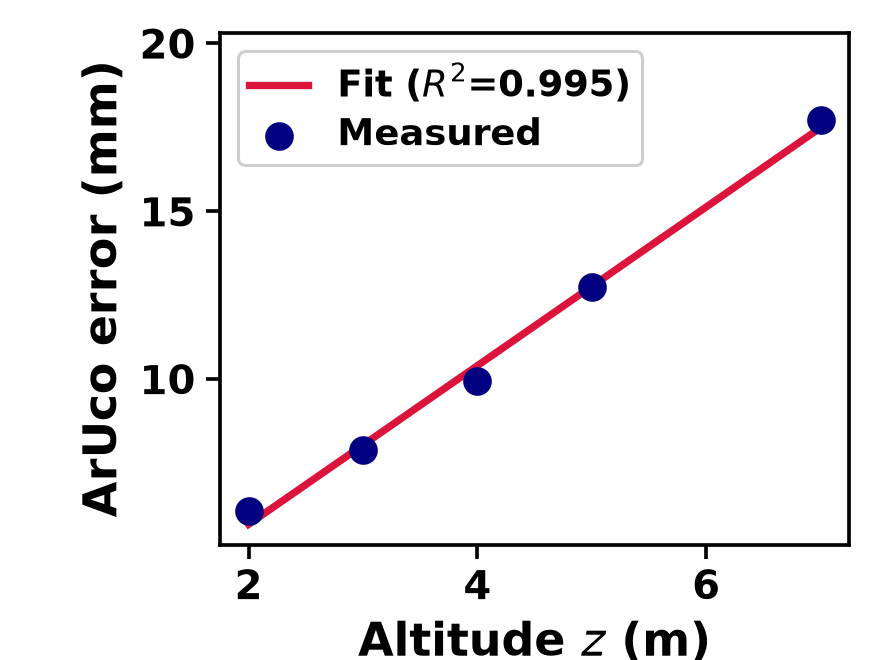
\includegraphics[width=0.5\columnwidth]{media/fig_e0.png}
\caption{Resolution-model validation (static altitude sweep, marker on axis). The mean ArUco position
error grows linearly with altitude \eqref{eq:e0fit} ($R^2=0.995$), confirming the $R\propto z^2$ law of
\eqref{eq:Rgsd}. One altitude with an intermittent detection dropout is excluded from the fit.}
\label{fig:e0}
\end{figure}

\subsection{Estimation cost and navigation cost versus altitude}
\label{sec:res_env}
Lemma~\ref{lem:mono} predicts that the steady-state estimation cost $g(z)=\tr P_\infty(R(z))$ is
nondecreasing in altitude, and Proposition~\ref{prop:alt} builds the optimal-altitude result on top of
it. We verify the premise in closed loop by sweeping the commanded altitude over $[2.5,7]$\,m on the
Low-$\kappa$, Mid-$\kappa$, and High-$\kappa$ tracks with the GSD noise model active. The measured
steady-state covariance trace rises monotonically with altitude, from $\tr\Sigma=0.0059$ at $z=2.5$\,m to
$0.0105$ at $z=7$\,m (Fig.~\ref{fig:envelope}(b)), and at each altitude it is nearly independent of
the track: for example $\{0.0058,0.0060,0.0058\}$ across the three tracks at $z=2.5$\,m and
$\{0.0106,0.0105,0.0104\}$ at $z=7$\,m. This track-independence is exactly what the shared-camera model
predicts, since the estimation cost enters through $R(z)$ alone and not through path geometry. The
opposing consideration is navigation. The UGV steering effort needed to keep the lane segmented is
smallest at intermediate altitude and rises at both extremes (Fig.~\ref{fig:envelope}(a)): steeply as
altitude drops toward the coverage floor, where the shrinking footprint begins to drop the lookahead, and
mildly at high altitude, where the coarser sampling adds waypoint noise. It also rises with curvature at
every altitude. Estimation cost, by contrast, decreases monotonically as altitude falls. Together the two
express the coverage-resolution trade-off of \eqref{eq:Rgsd} and \eqref{eq:eta}: estimation favors low
altitude while coverage forbids flying below the floor, which is why the estimation-optimal altitude of
Proposition~\ref{prop:alt} flies as low as segmentation allows and climbs where the floor rises.

\begin{figure}[t]
\centering
\subfloat[Navigation Cost]{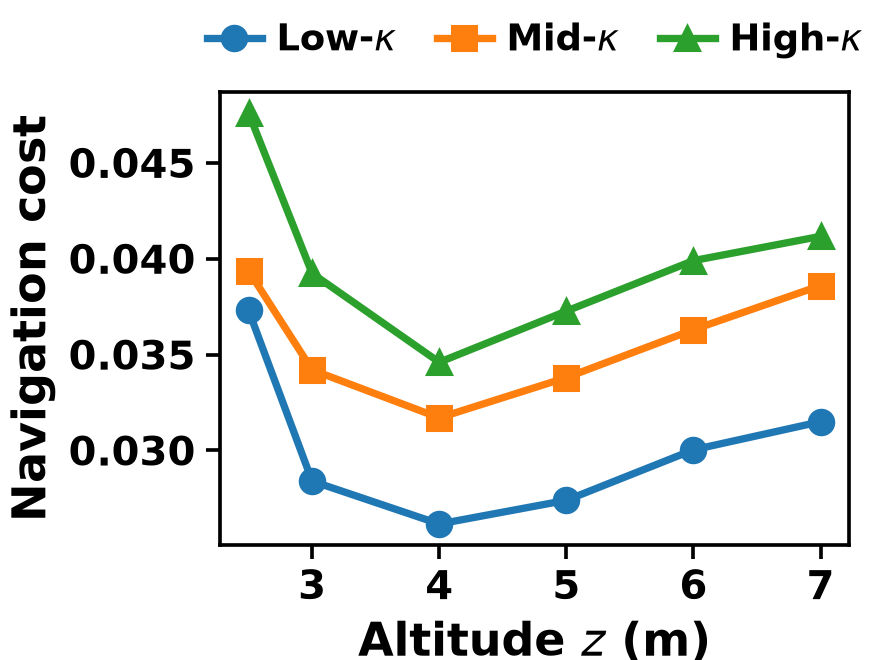
\includegraphics[width=0.49\columnwidth]{media/fig_env_nav.png}}\hfill
\subfloat[Estimation Cost]{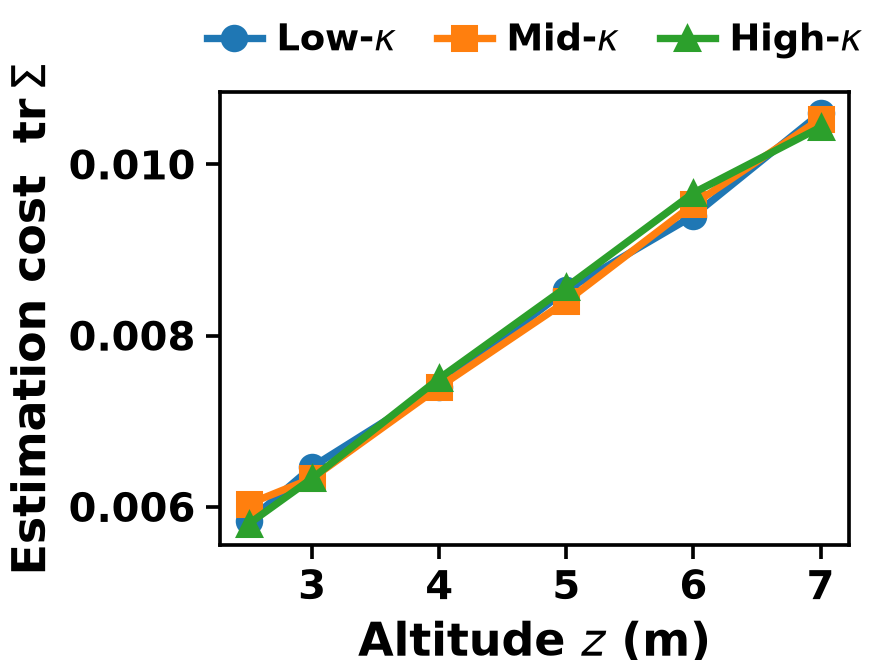
\includegraphics[width=0.49\columnwidth]{media/fig_env_cov.png}}
\caption{Coverage versus resolution across altitude. \textbf{(a)}~navigation (steering) cost is smallest
at intermediate altitude and rises at both extremes, growing with curvature $\kappa$. \textbf{(b)}~estimation
cost $\tr\Sigma$ grows monotonically with altitude (Lemma~\ref{lem:mono}) and is track-independent. The
optimum thus flies as low as coverage allows (Proposition~\ref{prop:alt}).}
\label{fig:envelope}
\end{figure}

\subsection{Altitude adaptation and its regime}
\label{sec:res_adapt}
Proposition~\ref{prop:adapt} gives a testable prediction: the curvature-scheduled policy strictly
beats every fixed altitude if and only if the coverage floor binds, $z_{\mathrm{fl}}(\kappa_{\max})>
z_{\min}$; otherwise it ties the lowest feasible fixed altitude, with gap $\Delta=0$. Our deployed
configuration sits on the non-binding side of the Corollary~\ref{cor:regime} boundary. The required
lookahead is $d_{\mathrm{look}}\approx0.5$\,m, so the floor is
$z_{\mathrm{fl}}\approx d_{\mathrm{look}}/\tan(\phi/2)\approx0.87$\,m, well below the actuation limit
$z_{\min}=2.5$\,m. The proposition therefore predicts $\Delta=0$ here, which is what the experiment
should show.

We run the policy against three fixed altitudes ($2.5$, $4.0$, and $7.0$\,m) on the Var-$\kappa$ track,
three repetitions each. The results match the prediction (Fig.~\ref{fig:altpolicy}):
\begin{itemize}
\item The adaptive policy attains mean $\tr\Sigma=0.0060$, only $2.8\%$ above the lowest fixed
altitude ($0.0058$ at $z=2.5$\,m), so $\Delta\approx0$;
\item The fixed-altitude cost rises monotonically with height, $0.0058\to0.0074\to0.0104$ from $2.5$ to
$7$\,m, a $79\%$ estimation penalty at the top, exactly the $g(z)$ increase of Lemma~\ref{lem:mono};
\item The adaptive altitude is not constant: it holds near the floor on straights and climbs to $3.9$\,m
through the sharpest turns, the ``climb into turns'' behavior of Corollary~\ref{cor:climb} emerging from
the coverage term rather than from a scripted maneuver;
\item Every configuration keeps the marker in view (ArUco visibility $\ge99\%$, no off-corridor
waypoints), consistent with a regime in which even the lowest altitude has adequate coverage.
\end{itemize}
The small gap is not a failure but the proposition's prediction for this regime: with the floor below
$z_{\min}$, no fixed altitude is dominated, so adaptation essentially matches the best fixed choice, the
residual reflecting the curvature-driven climbs the policy still commands where coverage does not require
them, while still avoiding the estimation penalty any higher altitude pays. The complementary binding regime,
$z_{\mathrm{fl}}(\kappa_{\max})>z_{\min}$, where the gain turns strictly positive, is entered only by a
lookahead that scales with speed or curvature; we characterize it in closed form and leave its closed-loop
demonstration to future work.

\begin{figure}[t]
\centering
\subfloat[Altitude vs.\ Time]{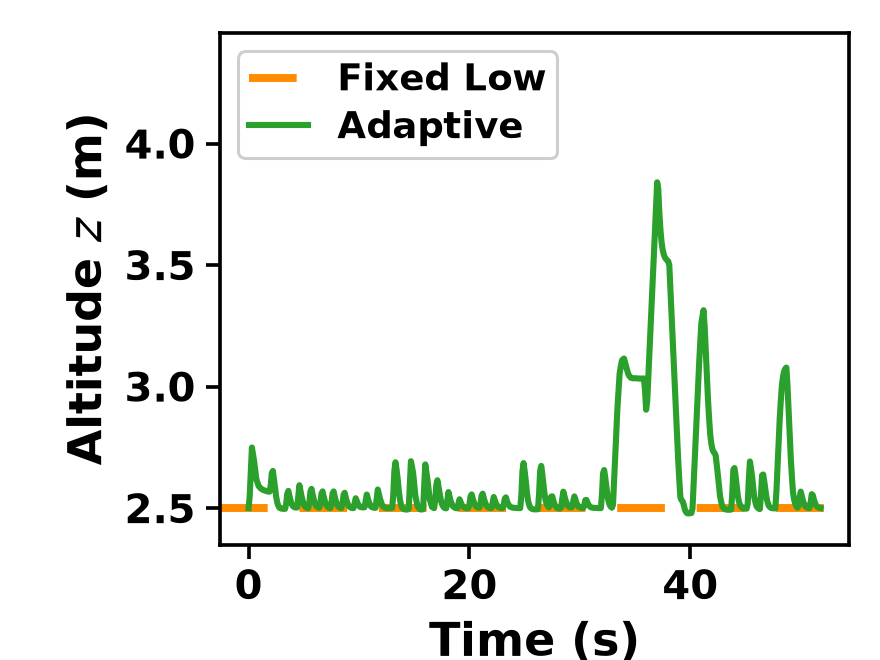
\includegraphics[width=0.49\columnwidth]{media/fig_alt_trace.png}}\hfill
\subfloat[Mean Estimation Cost]{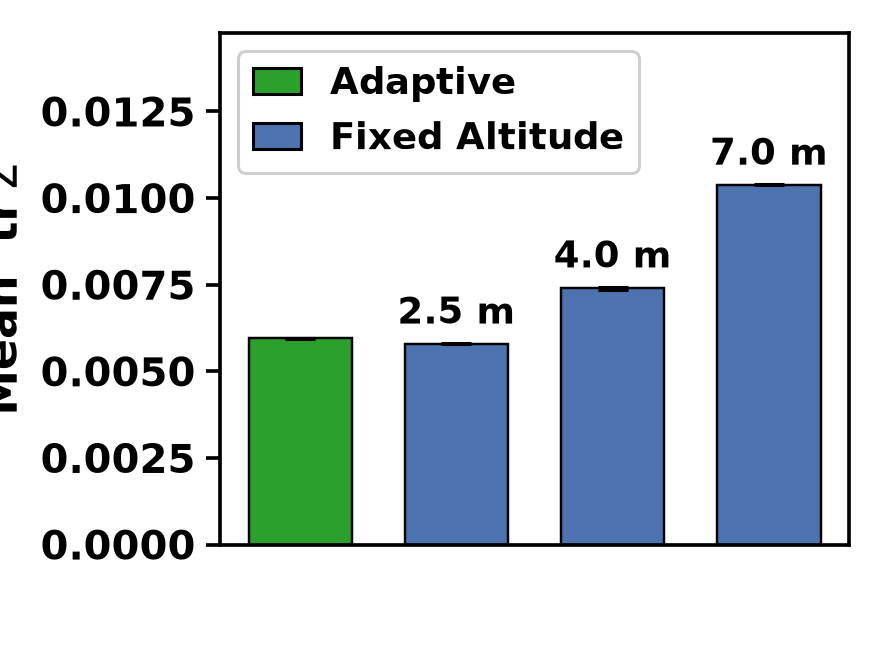
\includegraphics[width=0.49\columnwidth]{media/fig_cov_bars.png}}
\caption{Altitude adaptation in the non-binding regime (Var-$\kappa$ track, three repetitions).
\textbf{(a)}~the adaptive altitude holds near the floor on straights and climbs into turns
(Corollary~\ref{cor:climb}), spanning $[2.5,3.9]$\,m. \textbf{(b)}~mean estimation cost $\tr\Sigma$: the
adaptive policy matches the lowest fixed altitude ($\Delta\approx0$, as Proposition~\ref{prop:adapt}
predicts for $z_{\mathrm{fl}}<z_{\min}$), while higher fixed altitudes cost up to $79\%$ more.}
\label{fig:altpolicy}
\end{figure}

\subsection{Event-triggered co-design}
\label{sec:res_codesign}
Remark~\ref{rem:iss} shows that the perception-driven trigger fires without Zeno behavior and keeps the
inter-trigger error bounded, making it safe to replace continuous aerial replanning by event-triggered
replanning. The payoff is compute. Because the belief-space UGV
controller runs continuously in every configuration, the lever is the UAV nominal planner \eqref{eq:Ja};
we compare continuous replanning (C1) against the event-triggered scheme (C2) at a fixed altitude
($z=6$\,m), so that the compute effect is isolated from the altitude policy. Over three repetitions
(Table~\ref{tab:results}), C2 reduces aerial solves by $24.9\times$
($\RESsolvesCone\!\to\!\RESsolvesCthree$ per run) and aerial CPU by $12.3\times$
($\REScpuCone\!\to\!\REScpuCthree$\,ms per run), at matched estimation quality: the steady-state
covariance trace is $\REScov$ for both schemes and ArUco visibility is $\approx99.9\%$ for both. Each
individual C2 solve costs about twice as much ($\RESmsCthree$ vs.\ $\RESmsCone$\,ms), because it
re-optimizes from a shifted nominal trajectory, but the near $25$-fold reduction in the number of solves
dominates by an order of magnitude. The firings are dominated by curvature-anticipation events with
occasional plan-expiry events, and the re-plan rate stays bounded, consistent with Remark~\ref{rem:iss}.
This realizes the deployability requirement (iii) of Section~\ref{sec:problem}, perception-aware aerial
replanning at the cost of an occasional solve rather than a continuous one.

\begin{table}[h]
\caption{Aerial-planner co-design (fixed altitude $z=6$\,m, mean\,$\pm$\,std over three repetitions). C1
continuous vs.\ C2 event-triggered; the belief-space UGV controller runs continuously in both.
Steady-state window $t\!\ge\!8$\,s.}
\label{tab:results}
\begin{center}
\footnotesize
\setlength{\tabcolsep}{3pt}
\begin{tabular}{|l|c|c|}
\hline
{\textbf{Metric}} & {\textbf{C1 (cont.)}} & {\textbf{C2 (event)}}\\
\hline
Aerial solves (\#/run) & \RESsolvesCone & \RESsolvesCthree\\
\hline
Mean solve (ms) & \RESmsCone & \RESmsCthree\\
\hline
Aerial CPU (ms/run) & \REScpuCone & \REScpuCthree\\
\hline
Steady-state $\tr\Sigma$ & \REScov & \REScov\\
\hline
ArUco vis.\ (\%) & $\approx99.9$ & $\approx99.9$\\
\hline
UAV--UGV offset (m) & \RESoffCone & \RESoffCthree\\
\hline
\end{tabular}
\end{center}
\end{table}

\section{Conclusion and Future Work}
We studied aerial-ground cooperative tracking in which a single downward UAV camera is the ground
vehicle's only exteroceptive sensor, serving at once as its navigation reference and as the input to its
state estimator. The central observation is that this shared-sensor design couples navigation and
estimation through one scalar, the UAV altitude, which sets footprint coverage and localization resolution
in competition: flying lower sharpens localization but shrinks the footprint, while flying higher does the
reverse. We treated altitude as a variable to be optimized and solved this coupling in closed form. The
altitude that is best for estimation is the lowest one that keeps the path within the camera footprint, and
it rises with path curvature (Proposition~\ref{prop:alt}); adapting altitude beats every fixed altitude
exactly when this lowest admissible altitude is active and the curvature varies (Proposition~\ref{prop:adapt}),
and otherwise a fixed altitude is already optimal. We realized this as COAST, a perception-triggered
co-design whose ancillary law keeps the inter-trigger error bounded and free of Zeno behavior
(Remark~\ref{rem:iss}). A reproducible SITL study confirmed every prediction: the sensor noise follows
$R\propto z^2$; the estimation cost is monotone and track-independent in altitude; the adaptive policy
matches the best fixed altitude on our testbed while avoiding the penalty of flying higher; and
event-triggering the aerial planner reduces its computation by more than an order of magnitude at matched
estimation quality (Table~\ref{tab:results}). The contribution is the characterization of \emph{when}
altitude adaptation helps, not any single altitude value.

Future work will demonstrate the predicted strict benefit in the binding regime, reached by a speed- or
curvature-scaled look-ahead that lifts the coverage floor above $z_{\min}$, and will replace the
velocity-controlled UAV abstraction with a full multicopter model on hardware.

\bibliography{references}            % IFAC ifacconf.bst (author-year); see references.bib
\end{document}
